\documentclass[10pt, aspectratio=169]{beamer}

% --- Theme & Colors ---
\usetheme{Singapore}
\usecolortheme{default}

% --- Navigation & Page Numbering Setup ---
% 1. Remove standard bottom navigation symbols (arrows)
\setbeamertemplate{navigation symbols}{}

% 2. Add page numbering (Slide X / Y) to the bottom right
\setbeamertemplate{footline}{%
    \hfill%
    \usebeamercolor[fg]{page number in head/foot}%
    \usebeamerfont{page number in head/foot}%
    \insertframenumber\,/\,\inserttotalframenumber\kern1em\vskip2pt%
}

% --- Packages ---
\usepackage[utf8]{inputenc}
\usepackage{amsmath, amssymb, amsfonts}
\usepackage{graphicx}
\usepackage{booktabs}
\usepackage{microtype}
\usepackage{hyperref}
\usepackage{tikz}
\usetikzlibrary{positioning, arrows.meta, shapes.geometric, calc, backgrounds, fit}

% Write the bibliography file directly
\usepackage{filecontents}
\begin{filecontents}{references.bib}
@article{Brooks_2011,
   title={Handbook of Markov Chain Monte Carlo},
   publisher={Chapman and Hall/CRC},
   author={Brooks, Steve and Gelman, Andrew and Jones, Galin and Meng, Xiao-Li},
   year={2011}
}
@article{Yang_2021,
   title={B-PINNs: Bayesian physics-informed neural networks for forward and inverse PDE problems with noisy data},
   volume={425},
   journal={Journal of Computational Physics},
   publisher={Elsevier BV},
   author={Yang, Liu and Meng, Xuhui and Karniadakis, George Em},
   year={2021},
   pages={109913}
}
@misc{lakshminarayanan2017simplescalablepredictiveuncertainty,
      title={Simple and Scalable Predictive Uncertainty Estimation using Deep Ensembles}, 
      author={Balaji Lakshminarayanan and Alexander Pritzel and Charles Blundell},
      year={2017},
      archivePrefix={arXiv}
}
@article{NLL,
 author = {Lakshminarayanan, Balaji and Pritzel, Alexander and Blundell, Charles},
 title = {Simple and Scalable Predictive Uncertainty Estimation using Deep Ensembles},
 volume = {30},
 year = {2017}
}
@article{picp_mpiw,
  author={Khosravi, Abbas and Nahavandi, Saeid and Creighton, Doug and Atiya, Amir F.},
  journal={IEEE Transactions on Neural Networks}, 
  title={Comprehensive Review of Neural Network-Based Prediction Intervals and New Advances}, 
  year={2011},
  volume={22},
  number={9},
  pages={1341-1356}
}
@inproceedings{ECE,
  title = {On Calibration of Modern Neural Networks},
  author = {Chuan Guo and Geoff Pleiss and Yu Sun and Kilian Q. Weinberger},
  booktitle = {Proceedings of the 34th International Conference on Machine Learning},
  pages = {1321--1330},
  year = {2017},
  volume = {70}
}
@inproceedings{Lee2018,
  title={Deep Neural Networks as Gaussian Processes},
  author={Jaehoon Lee and Yasaman Bahri and Roman Novak and Samuel S. Schoenholz and Jeffrey Pennington and Jascha Sohl-Dickstein},
  booktitle={International Conference on Learning Representations},
  year={2018}
}
\end{filecontents}

% Metadata
\title[Bayesian PINNs]{Bayesian Physics-Informed Neural Networks}
\author[Ruer, Ifrah, Forcioli]{Anouk Ruer \and Ruben Ifrah \and P\'en\'elope Forcioli}
\institute[]{Université Paris Dauphine - PSL\\ 
\includegraphics[height=3cm]{Figures/LOGO-PSL-nov-2017.png}}
\date{2024}

\begin{document}

% Slide 1: Title
\begin{frame}
    \titlepage
\end{frame}

% =========================================================================
% B-PINNs Presentation — Paper slides only (no extension)
% 5 slides, ~6 minutes
% =========================================================================

\section*{Introduction}

% -------------------------------------------------------------------
% Slide 0: Physics-Informed Neural Networks (PINNs)
% -------------------------------------------------------------------
\begin{frame}{Physics-Informed Neural Networks (PINNs)}
    \begin{columns}
        \begin{column}{0.5\textwidth}
            \textbf{General PDE setup:}
            \[
                \mathcal{N}_x(u;\lambda) = f \text{ on } D, \;\;
                \mathcal{B}_x(u;\lambda) = b \text{ on } \Gamma
            \]
            where $\mathcal{N}_x$ is a differential operator, $\lambda$ are PDE parameters, $f$ is the forcing term, and $\mathcal{B}_x$ is the boundary operator.
            
            \vspace{0.3cm}
            \textbf{Observational Data:}
            Dataset $\mathcal{D} = \mathcal{D}_u \cup \mathcal{D}_f \cup \mathcal{D}_b$ of noisy sensor measurements:
            \begin{itemize}
                \item $\mathcal{D}_u$: measurements of sol $u$
                \item $\mathcal{D}_f$: measurements of forcing $f$
                \item $\mathcal{D}_b$: measurements of b.c. $b$
            \end{itemize}
            Measurements corrupted by Gaussian noise:
            \[ \bar{u}^{(i)} = u(\boldsymbol{x}_u^{(i)}) + \epsilon_u^{(i)}, \epsilon \sim \mathcal{N}(0, \sigma^2) \]
        \end{column}
        \begin{column}{0.5\textwidth}
            \begin{figure}
                \centering
                
\includegraphics[width=\textwidth]{Figures/intro_pinn_data.png}
                \caption{Example of observational data points sampled from the domain and boundaries.}
            \end{figure}
        \end{column}
    \end{columns}
\end{frame}

% -------------------------------------------------------------------
% Slide 1: Motivation & Problem Statement
% -------------------------------------------------------------------
\begin{frame}{Motivation \& Problem Statement}
    \textbf{Standard PINNs:}
    \begin{itemize}
        \item Learn PDE solutions using limited data and physical laws via deterministic gradient descent.
        \item \textbf{Limitation:} They lack built-in uncertainty quantification and are highly prone to overfitting when sensor data is noisy.
    \end{itemize}
    \vspace{0.5cm}
    \textbf{The Solution: Bayesian PINNs (B-PINNs) \cite{Yang_2021}}
    \begin{itemize}
        \item Extend standard PINNs into a Bayesian framework.
        \item Treat neural network weights probabilistically rather than as fixed values.
        \item Yields a \textit{distribution} of possible solutions, providing natural uncertainty quantification.
    \end{itemize}
\end{frame}

\section{The B-PINN Framework}

% -------------------------------------------------------------------
% Slide 2: The B-PINN Framework
% -------------------------------------------------------------------
\begin{frame}{The B-PINN Framework}

    \textbf{General PDE setup:}
    \[
        \mathcal{N}_x(u;\lambda) = f, \qquad
        \mathcal{B}_x(u;\lambda) = b
    \]
    Dataset $\mathcal{D} = \mathcal{D}_u \cup \mathcal{D}_f \cup \mathcal{D}_b$ 
    of noisy sensor measurements:
    \[
        \bar{u}^{(i)} = u(\boldsymbol{x}_u^{(i)}) + \epsilon_u^{(i)}, \quad
        \bar{f}^{(i)} = f(\boldsymbol{x}_f^{(i)}) + \epsilon_f^{(i)}, \quad
        \bar{b}^{(i)} = f(\boldsymbol{x}_b^{(i)}) + \epsilon_b^{(i)}, \quad
        \epsilon \sim \mathcal{N}(0, \sigma^2)
    \]

    \vspace{0.3cm}
    \textbf{BNN surrogate} $\tilde{u}(x;\boldsymbol{\theta})$ approximates $u$, 
    from which $f$ and $b$ are derived via automatic differentiation:
    \[
        \tilde{f}(x;\boldsymbol{\theta}) = \mathcal{N}_x(\tilde{u}(x;\boldsymbol{\theta});\lambda),
        \qquad
        \tilde{b}(x;\boldsymbol{\theta}) = \mathcal{B}_x(\tilde{u}(x;\boldsymbol{\theta});\lambda)
    \]

    \vspace{0.3cm}
    \textbf{Gaussian prior} A Gaussian prior is placed independently on each component of the network weights $\theta$;  
    $P(\boldsymbol{\theta}) = \mathcal{N}(\boldsymbol{0}, \boldsymbol{I})$

    \vspace{0.2cm}
    \textbf{Posterior} by Bayes' theorem:
    \[
        P(\boldsymbol{\theta} \mid \mathcal{D}) \;\propto\; 
        \underbrace{P(\mathcal{D} \mid \boldsymbol{\theta})}_{\text{physics-informed likelihood}} 
        \cdot 
        P(\boldsymbol{\theta})
    \]

\end{frame}

% -------------------------------------------------------------------
% Slide 3: Posterior Sampling Approaches
% -------------------------------------------------------------------
\begin{frame}{Posterior Sampling Approaches}
    \vspace{0.3cm}
    \textbf{1. Hamiltonian Monte Carlo (HMC)}
    \begin{itemize}
        \item Introduces auxiliary momentum variable; simulates Hamiltonian dynamics.
        \item Makes large, informed moves — avoids random-walk behavior.
        \item \textbf{Asymptotically exact} samples from the true posterior.
        \item Cost: computationally expensive.
    \end{itemize}

    \vspace{0.3cm}
    \textbf{2. Variational Inference (VI)}
    \begin{itemize}
        \item Recasts inference as optimisation — minimises KL divergence.
        \item Fits a \textbf{fully factorised Gaussian}: each weight assumed independent.
        \item Fast, but the mean-field assumption \textbf{underestimates posterior variance} — overconfident under high noise.
    \end{itemize}
    
    The Dropout is introduced as a cheap baseline.\and
\end{frame}

% -------------------------------------------------------------------
% Slide 4: Results — Forward Problem
% -------------------------------------------------------------------
\begin{frame}{Key Findings from the Baseline Study}
    \begin{figure}{\textwidth} 
        \centering
        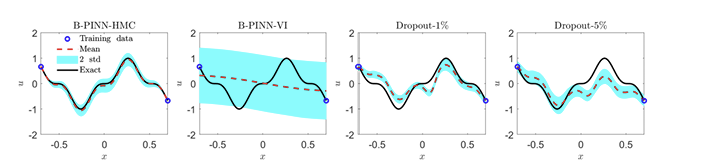
\includegraphics[width=\linewidth]{Figures/picture_paper.png}
    \end{figure}
    Systematic comparison of standard PINNs, B-PINN (HMC \& VI), and Dropout:
    \vspace{0.3cm}
    \begin{itemize}
        \item \textbf{B-PINN-HMC Excels:} Consistently delivers reliable predictive means and correctly calibrated uncertainty bounds across noise scales.
        \item \textbf{VI Fails:} Factorizable Gaussian assumptions restrict weights from correlating, leading to severely degraded uncertainty quantification.
        \item \textbf{Overfitting Protection:} Under large noise ($\sigma = 0.1$), B-PINN-HMC acts as a regularizer where deterministic PINNs catastrophically overfit.
    \end{itemize}
\end{frame}



% PENEWWWWWWW -- -- -- -- -- -- -- -- -- -- -- --
\begin{frame}{Metrics for Uncertainty Quantification}
    Visual checks are insufficient for Bayesian methods. We utilize uncertainty-aware metrics:
    \begin{itemize}
        \item \textbf{PICP} (Prediction Interval Coverage): Fraction of true data captured by bounds.
        $\text{PICP} = \frac{1}{N} \sum_{i=1}^{N} c_i, \quad c_i = \mathbb{I}(L_i \le y_{true, i} \le U_i)$
        \item \textbf{MPIW} (Mean Prediction Interval Width): Average width of the $\pm 2\sigma$ bands.
        $\text{MPIW} = \frac{1}{N} \sum_{i=1}^{N} (U_i - L_i)$
        \item \textbf{NLL} (Negative Log-Likelihood): Penalizes "confidently wrong" models.
        \[ \text{NLL} = \frac{1}{N} \sum_{i=1}^{N} \left( \frac{\log(2\pi\sigma_i^2)}{2} + \frac{(y_i - \mu_i)^2}{2\sigma_i^2} \right) \]
        \item \textbf{ECE} (Expected Calibration Error): Weighted average of bin-wise error.
        \[ \text{ECE} = \sum_{m=1}^{M} \frac{|B_m|}{N} \left| \text{acc}(B_m) - \text{conf}(B_m) \right| \]
    \end{itemize}
\end{frame}

% Slide 7
\begin{frame}{B-PINNs with Unknown Noise}
    \textbf{The Unrealistic Assumption:}
    \begin{itemize}
        \item Standard models assume the noise level $\sigma_f$ is perfectly known. In real physics scenarios, this is rarely true.
    \end{itemize}
    \vspace{0.3cm}
    \textbf{Our Fix: Hierarchical B-PINNs}
    \begin{itemize}
        \item We assigned a log-normal prior to the noise and jointly inferred it alongside network weights using HMC.
        \item \textbf{Mathematical Adjustment:} The normalization constant cannot be dropped. The log-likelihood must explicitly retain the variance penalty:
        $$ \log P(\mathcal{D}_f | \theta, \psi) \propto -N_f \psi - \frac{SSE_f(\theta)}{2 \exp(2\psi)} $$
        where $\psi = \log \sigma_f$.
    \end{itemize}
\end{frame}

\section{Experimental Results}

\begin{frame}{Experimental Results: 1D Poisson equation ($\lambda u_{xx} = f(x)$)}

\begin{figure}
\centering
\begin{tabular}{@{}cccc@{}}
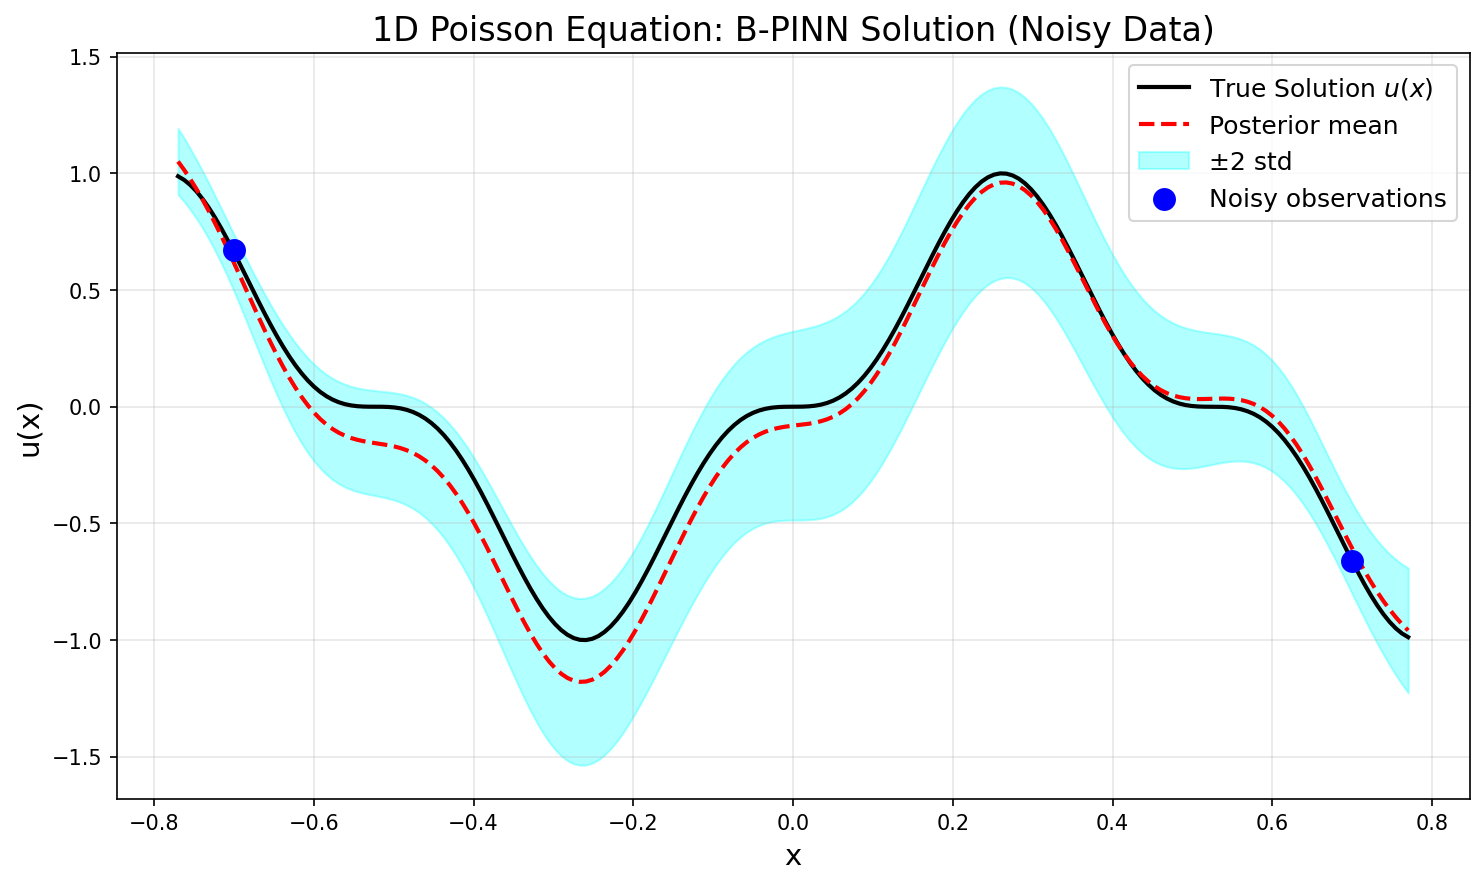
\includegraphics[width=0.22\textwidth]{Figures/1D poisson sigma = 0.01/BPINN.png} &
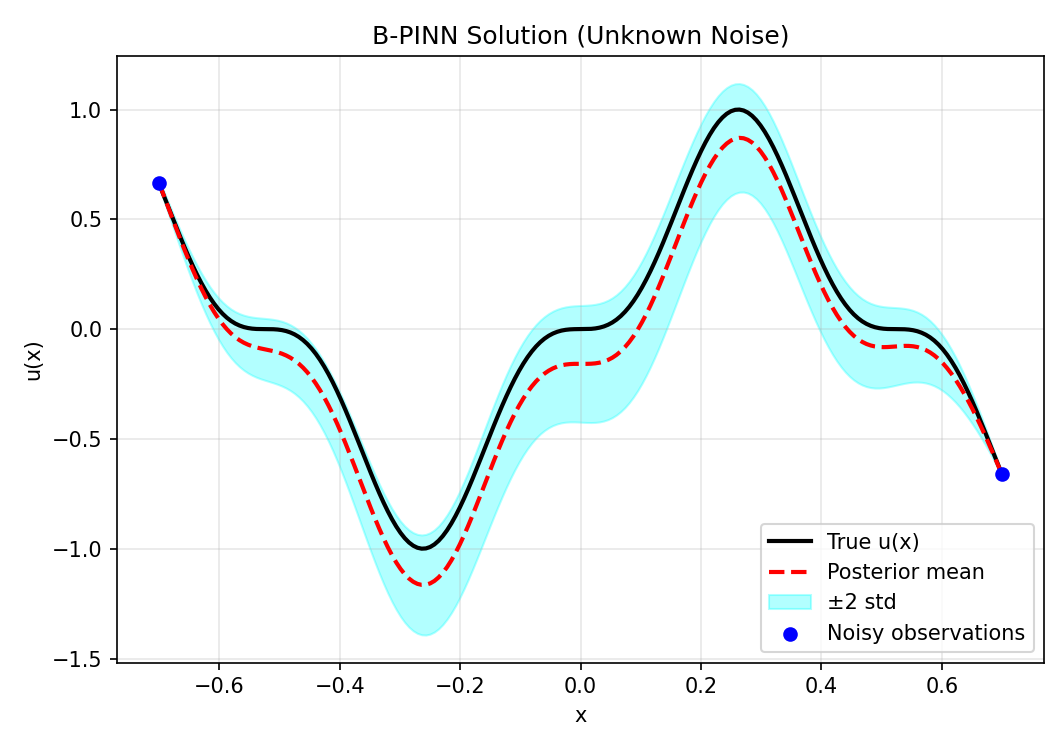
\includegraphics[width=0.22\textwidth]{Figures/1D poisson sigma = 0.01/HBPINN_modif.png} &
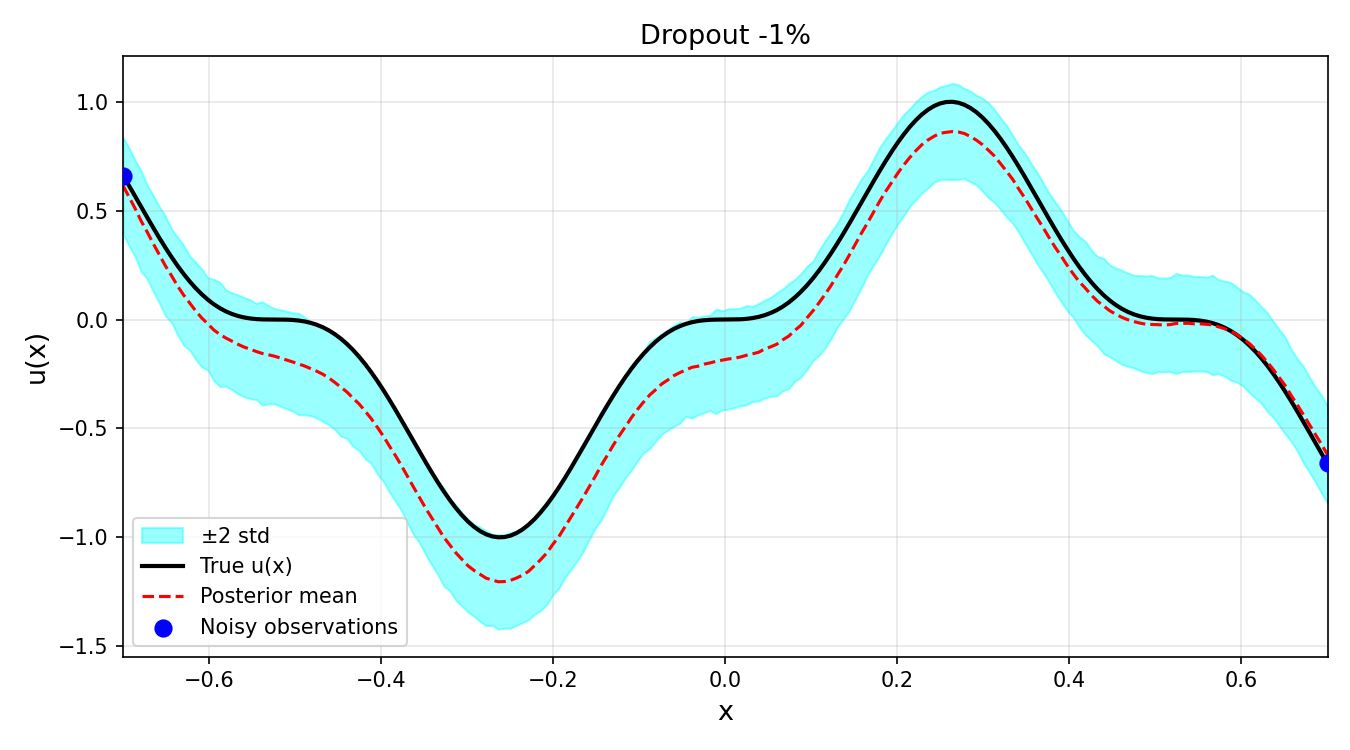
\includegraphics[width=0.22\textwidth]{Figures/dropout/dropout_1_01.png} &
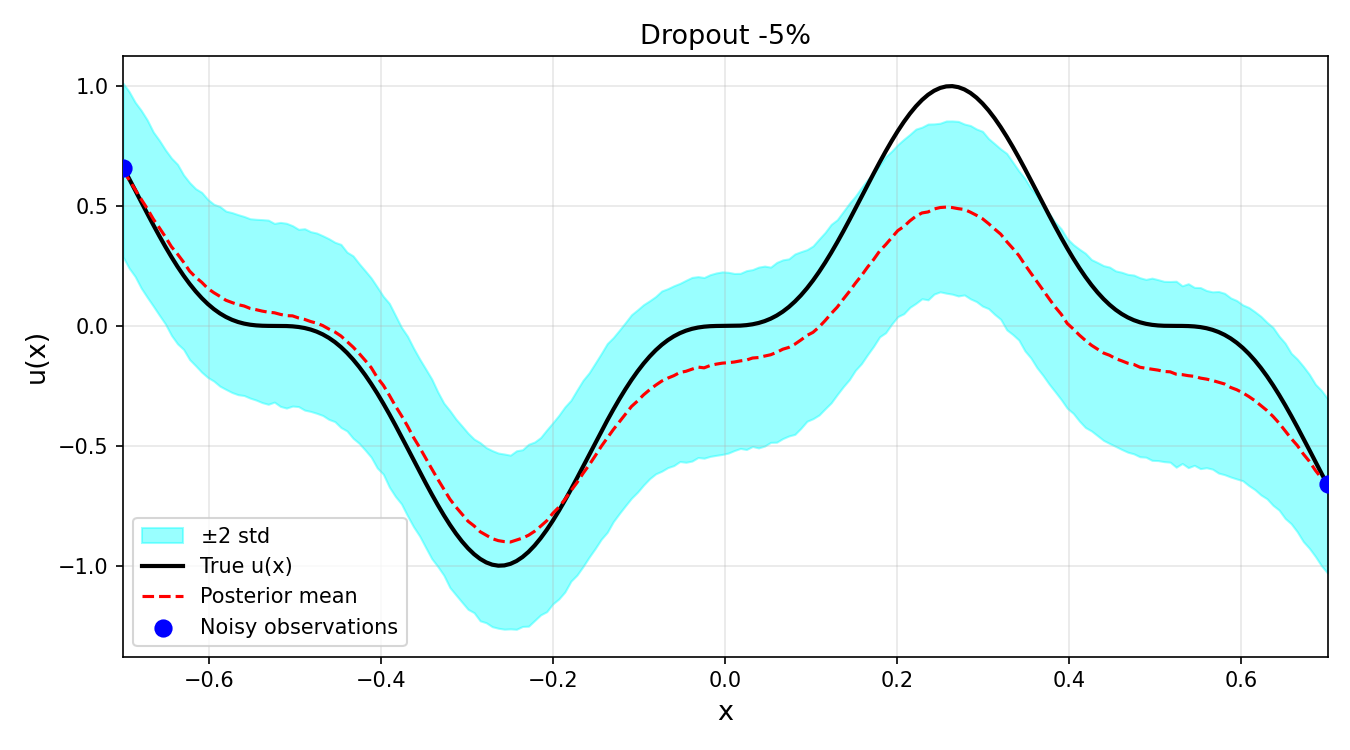
\includegraphics[width=0.22\textwidth]{Figures/dropout/dropout_5_01.png} \\
\scriptsize (a) BPINN & \scriptsize (b) BPINN w prior & \scriptsize (c) Dropout 1\% & \scriptsize (d) Dropout 5\% \\
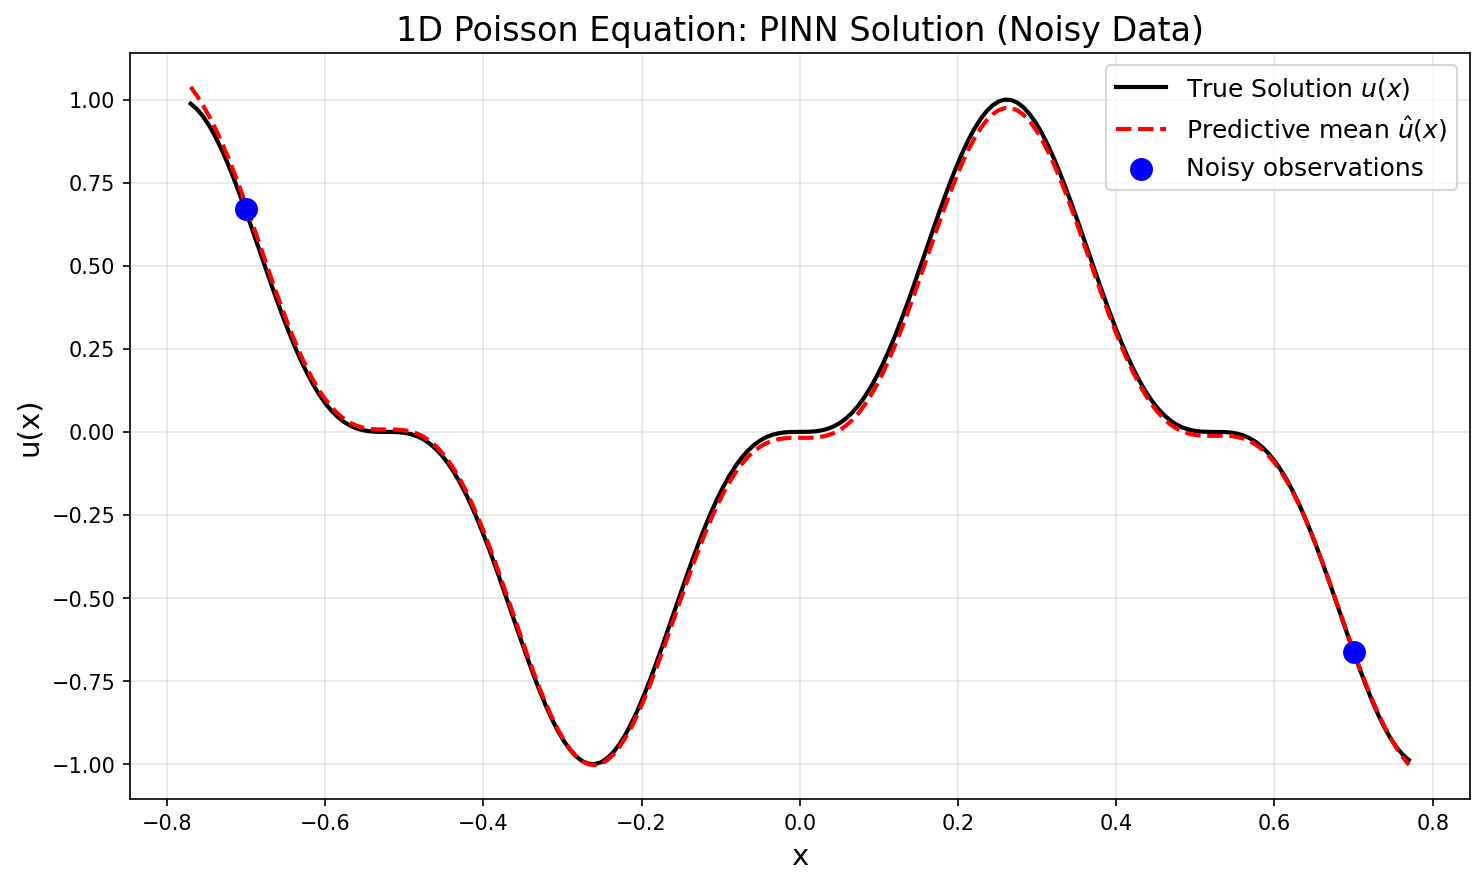
\includegraphics[width=0.22\textwidth]{Figures/1D poisson sigma = 0.01/PINN.png} \\
\scriptsize (e) PINN
% Add more images here if needed, or leave empty for now
\end{tabular}
\end{figure}

\end{frame}


\begin{frame}{Experimental Results: 1D Poisson equation ($\lambda u_{xx} = f(x)$) (1)}

  
\begin{table}[h]
\centering
\resizebox{0.45\textwidth}{!}{%
\begin{tabular}{|c|c|c|c|c|c|}
\hline
 & B-PINN & B-PINN (unknown noise)  & PINN & Dropout -5\% & Dropout - 1\%  \\
\hline
Relative $L^2$ norm & 0.2952  & 0.2251  &   0.4338 & 0.3644 &0.3713 \\
\hline
PICP & 92.60 & 100 & - & 95.50 & 54.00 \\
\hline
MPIW & 0.6465 & 0.7137 & - & 0.7864 & 0.4048 \\
\hline
NLL & -0.3885 & -0.7345 & - & -0.2677 & 0.3478 \\
\hline
ECE &  0.1307 & 0.1016 & -  & 0.0374 & 0.3090 \\
\hline
\end{tabular}}
\caption{\tiny Metrics for the 1D poisson equation forward problem with measurement noise 0.1}
\label{tab:5x5}
\end{table}



\begin{table}[h]
\centering
\resizebox{0.45\textwidth}{!}{%
\begin{tabular}{|c|c|c|c|c|c|}
\hline
 & B-PINN & B-PINN (unknown noise)  & PINN & Dropout 5\% & Dropout 1\%   \\
\hline
Relative $L^2$ norm & 0.2220  & 0.2492  &   0.0324 & 0.4341 & 0.3059  \\
\hline
PICP( \%) & 100 & 100 & - & 86.00 & 95.50 \\
\hline
MPIW & 0.6389 & 0.3887 & - & 0.7398 & 0.4462 \\
\hline
NLL & -0.6452 & -0.8415  & - & -0.0357 & -0.3265 \\
\hline
ECE &  0.0640 & 0.2432 & - & 0.0367 & 0.1950\\
\hline
\end{tabular}}
\caption{ \tiny Metrics for the 1D poisson equation forward problem with measurement noise 0.01}
\label{tab:5x5}
\end{table}

\textbf{B-PINN vs. PINN under Noise Regimes}
\begin{itemize}
    \item High Noise: Standard PINNs overfit sensor noise, leading to high $L^2$ error. B-PINNs treat physics as "soft" constraints, filtering high-frequency noise to achieve a lower error of 0.2952.
    \item Low Noise: Standard PINNs excel by finding the global minimum of clean data. B-PINNs struggle to sample these "sharp" peaks via HMC, resulting in a slightly higher mean error of 0.2220.
\end{itemize}
\end{frame}

\begin{frame}{Experimental Results: 1D Poisson equation ($\lambda u_{xx} = f(x)$) (2)}

  
\begin{table}[h]
\centering
\resizebox{0.45\textwidth}{!}{%
\begin{tabular}{|c|c|c|c|c|c|}
\hline
 & B-PINN & B-PINN (unknown noise)  & PINN & Dropout -5\% & Dropout - 1\%  \\
\hline
Relative $L^2$ norm & 0.2952  & 0.2251  &   0.4338 & 0.3644 &0.3713 \\
\hline
PICP & 92.60 & 100 & - & 95.50 & 54.00 \\
\hline
MPIW & 0.6465 & 0.7137 & - & 0.7864 & 0.4048 \\
\hline
NLL & -0.3885 & -0.7345 & - & -0.2677 & 0.3478 \\
\hline
ECE &  0.1307 & 0.1016 & -  & 0.0374 & 0.3090 \\
\hline
\end{tabular}}
\caption{\tiny Metrics for the 1D poisson equation forward problem with measurement noise 0.1}
\label{tab:5x5}
\end{table}



\begin{table}[h]
\centering
\resizebox{0.45\textwidth}{!}{%
\begin{tabular}{|c|c|c|c|c|c|}
\hline
 & B-PINN & B-PINN (unknown noise)  & PINN & Dropout 5\% & Dropout 1\%   \\
\hline
Relative $L^2$ norm & 0.2220  & 0.2492  &   0.0324 & 0.4341 & 0.3059  \\
\hline
PICP( \%) & 100 & 100 & - & 86.00 & 95.50 \\
\hline
MPIW & 0.6389 & 0.3887 & - & 0.7398 & 0.4462 \\
\hline
NLL & -0.6452 & -0.8415  & - & -0.0357 & -0.3265 \\
\hline
ECE &  0.0640 & 0.2432 & - & 0.0367 & 0.1950\\
\hline
\end{tabular}}
\caption{ \tiny Metrics for the 1D poisson equation forward problem with measurement noise 0.01}
\label{tab:5x5}
\end{table}





\textbf{The behaviour of the B-PINN with a noise prior}
\begin{itemize}
    \item High Noise: Superior performance. The inferred noise parameter ($\sigma_f$) acts as an adaptive weight, allowing the model to prioritize physical consistency over noisy contradictory data.
    \item Low Noise: Although the model overestimates the $0.01$ noise scale, it ensures robustness. This dynamic parameter prevents HMC divergence by avoiding "numerical traps" caused by overly sharp posteriors, maintaining 100\% coverage.
    \end{itemize}
\end{frame}


\begin{frame}{Experimental Results: 1D Poisson equation ($\lambda u_{xx} = f(x)$) (3)}

  
\begin{table}[h]
\centering
\resizebox{0.45\textwidth}{!}{%
\begin{tabular}{|c|c|c|c|c|c|}
\hline
 & B-PINN & B-PINN (unknown noise)  & PINN & Dropout -5\% & Dropout - 1\%  \\
\hline
Relative $L^2$ norm & 0.2952  & 0.2251  &   0.4338 & 0.3644 &0.3713 \\
\hline
PICP & 92.60 & 100 & - & 95.50 & 54.00 \\
\hline
MPIW & 0.6465 & 0.7137 & - & 0.7864 & 0.4048 \\
\hline
NLL & -0.3885 & -0.7345 & - & -0.2677 & 0.3478 \\
\hline
ECE &  0.1307 & 0.1016 & -  & 0.0374 & 0.3090 \\
\hline
\end{tabular}}
\caption{\tiny Metrics for the 1D poisson equation forward problem with measurement noise 0.1}
\label{tab:5x5}
\end{table}



\begin{table}[h]
\centering
\resizebox{0.45\textwidth}{!}{%
\begin{tabular}{|c|c|c|c|c|c|}
\hline
 & B-PINN & B-PINN (unknown noise)  & PINN & Dropout 5\% & Dropout 1\%   \\
\hline
Relative $L^2$ norm & 0.2220  & 0.2492  &   0.0324 & 0.4341 & 0.3059  \\
\hline
PICP( \%) & 100 & 100 & - & 86.00 & 95.50 \\
\hline
MPIW & 0.6389 & 0.3887 & - & 0.7398 & 0.4462 \\
\hline
NLL & -0.6452 & -0.8415  & - & -0.0357 & -0.3265 \\
\hline
ECE &  0.0640 & 0.2432 & - & 0.0367 & 0.1950\\
\hline
\end{tabular}}
\caption{ \tiny Metrics for the 1D poisson equation forward problem with measurement noise 0.01}
\label{tab:5x5}
\end{table}




\textbf{The impact of the prior on the noise on the uncertainty}
    \begin{itemize}
        \item Produces wider, more conservative bands (MPIW 0.7137) at high noise than the vanilla B-PINN
        \item In low noise, it produces tighter intervals than vanilla B-PINN (0.3887 vs 0.6389), possibly because of a better HMC behaviour due to its inflated noise estimation
    \end{itemize}
\textbf{Dropout Failure}
\begin{itemize}
    \item  Dropout bands are dictated by the \textit{rate}, not the \textit{data}.
    \end{itemize}
\end{frame}


  
\section{from B-PINNs to PI-GP}

\begin{frame}{Theoretical Motivation: The PI-GP Baseline}
    \textbf{Why compare B-PINNs with Gaussian Processes?}
    \begin{itemize}
        \item Finite-width B-PINNs completely depend on approximate sampling (HMC, VI) over a highly non-convex posterior energy landscape: $U(\theta) = -\log P(\mathcal{D}\mid\theta) - \log P(\theta)$.
        \item Sampling depends heavily on hyper-parameter tuning and lacks simple analytical performance guarantees.
    \end{itemize}
    \vspace{0.1cm}
    \begin{block}{Establishing an Absolute Ground-Truth Baseline}
        \begin{itemize}
            \item By the Central Limit Theorem, in the infinite-width limit $N_l \to \infty$, a BNN prior converges to a \textbf{Neural Network Gaussian Process (NNGP)}: $u(\cdot;\theta) \xrightarrow{\text{Dist.}} \mathcal{GP}\big(0, k_{\text{NNGP}}(\cdot, \cdot)\big)$.
            \item If the differential operators are \textbf{linear}, the B-PINN formulation analytically reduces to a \textbf{Physics-Informed Gaussian Process (PI-GP)}.
            \item The PI-GP bypasses sampling, allowing us to strictly benchmark the adaptivity of finite-width B-PINNs against exactly the mathematical limit they are derived from.
        \end{itemize}
    \end{block}
\end{frame}

\begin{frame}{The Infinite-Width Limit: BNNs as NNGPs}
    \textbf{From Neural Networks to Gaussian Processes:}
    \begin{itemize}
        \item Consider a fully-connected BNN surrogate $\tilde{u}(x; \theta)$ with hidden layers of width $N_l$.
        \item By the Central Limit Theorem, as the hidden layer widths $N_l \to \infty$, the pre-activations converge to a multivariate Gaussian. 
        \item Consequently, the \textbf{output surrogate function converges to a Gaussian Process}:
        \[
        u(\cdot;\theta) \xrightarrow[N_l \to \infty]{\text{Distribution}} \mathcal{GP}\big(0, k_{\text{NNGP}}(\cdot, \cdot)\big)
        \]
    \end{itemize}
    \vspace{0.2cm}
    \textbf{The Kernel $k_{\text{NNGP}}$:}
    \begin{itemize}
        \item The prior covariance kernel is recursively determined by the network depth, variance priors ($\sigma_w^2, \sigma_b^2$), and the activation function $\phi$:
        \[
        K^{(0)}(x, x') = \frac{\sigma_w^2}{d_{in}} x \cdot x' + \sigma_b^2 \quad \quad K^{(l)}(x, x') = \sigma_w^2 \mathbb{E}_{(z, z') \sim \mathcal{N}(0, \Sigma^{(l-1)})} \Big[ \phi(z) \phi(z') \Big] + \sigma_b^2
        \]
        \item \textbf{Implication:} An infinitely wide B-PINN prior induces an exact GP prior on the predicted solution field $u(\cdot)$.
    \end{itemize}
\end{frame}

\begin{frame}{Gaussian Processes under Linear Differential Operators}
    \textbf{The exact equations defining the PI-GP block Covariance $\mathbf{K}$:}
    \begin{itemize}
        \item If the differential operator $\mathcal{L}_x$ is \textbf{linear}, applying it to $u \sim \mathcal{GP}\big(0, k_{\text{NNGP}}(x, x')\big)$ yields a Gaussian Process. The spatial operators commute with the covariance expectation:
        \[
        \text{Cov}\big(u(x), \mathcal{L}_{x'} u(x')\big) = \mathcal{L}_{x'} k_{\text{NNGP}}(x, x')
        \]
        \[
        \text{Cov}\big(\mathcal{L}_x u(x), \mathcal{L}_{x'} u(x')\big) = \mathcal{L}_x \mathcal{L}_{x'} k_{\text{NNGP}}(x, x')
        \]
    \end{itemize}
    \textbf{Analytical PI-GP Posterior:}
    \begin{itemize}
        \item With data $\mathcal{D}$, the inference reduces to a \textbf{closed-form GP regression}:
        \begin{align*}
        \mu(x^*) &= \mathbf{k}_{*} (\mathbf{K} + \Sigma_{\text{noise}})^{-1} Y \\
        \Sigma(x^*) &= k(x^*, x^*) - \mathbf{k}_{*} (\mathbf{K} + \Sigma_{\text{noise}})^{-1} \mathbf{k}_{*}^T
        \end{align*}
        \item No more iterative neural network training and sometimes unstable MC sampling, yielding an exact, resolution-free, convex analytical ground-truth posterior.
    \end{itemize}
\end{frame}


\begin{frame}{Empirical Evaluation: Expressivity vs. Adaptivity}
    \begin{columns}
        \begin{column}{0.45\textwidth}
            \begin{figure} 
                \centering
                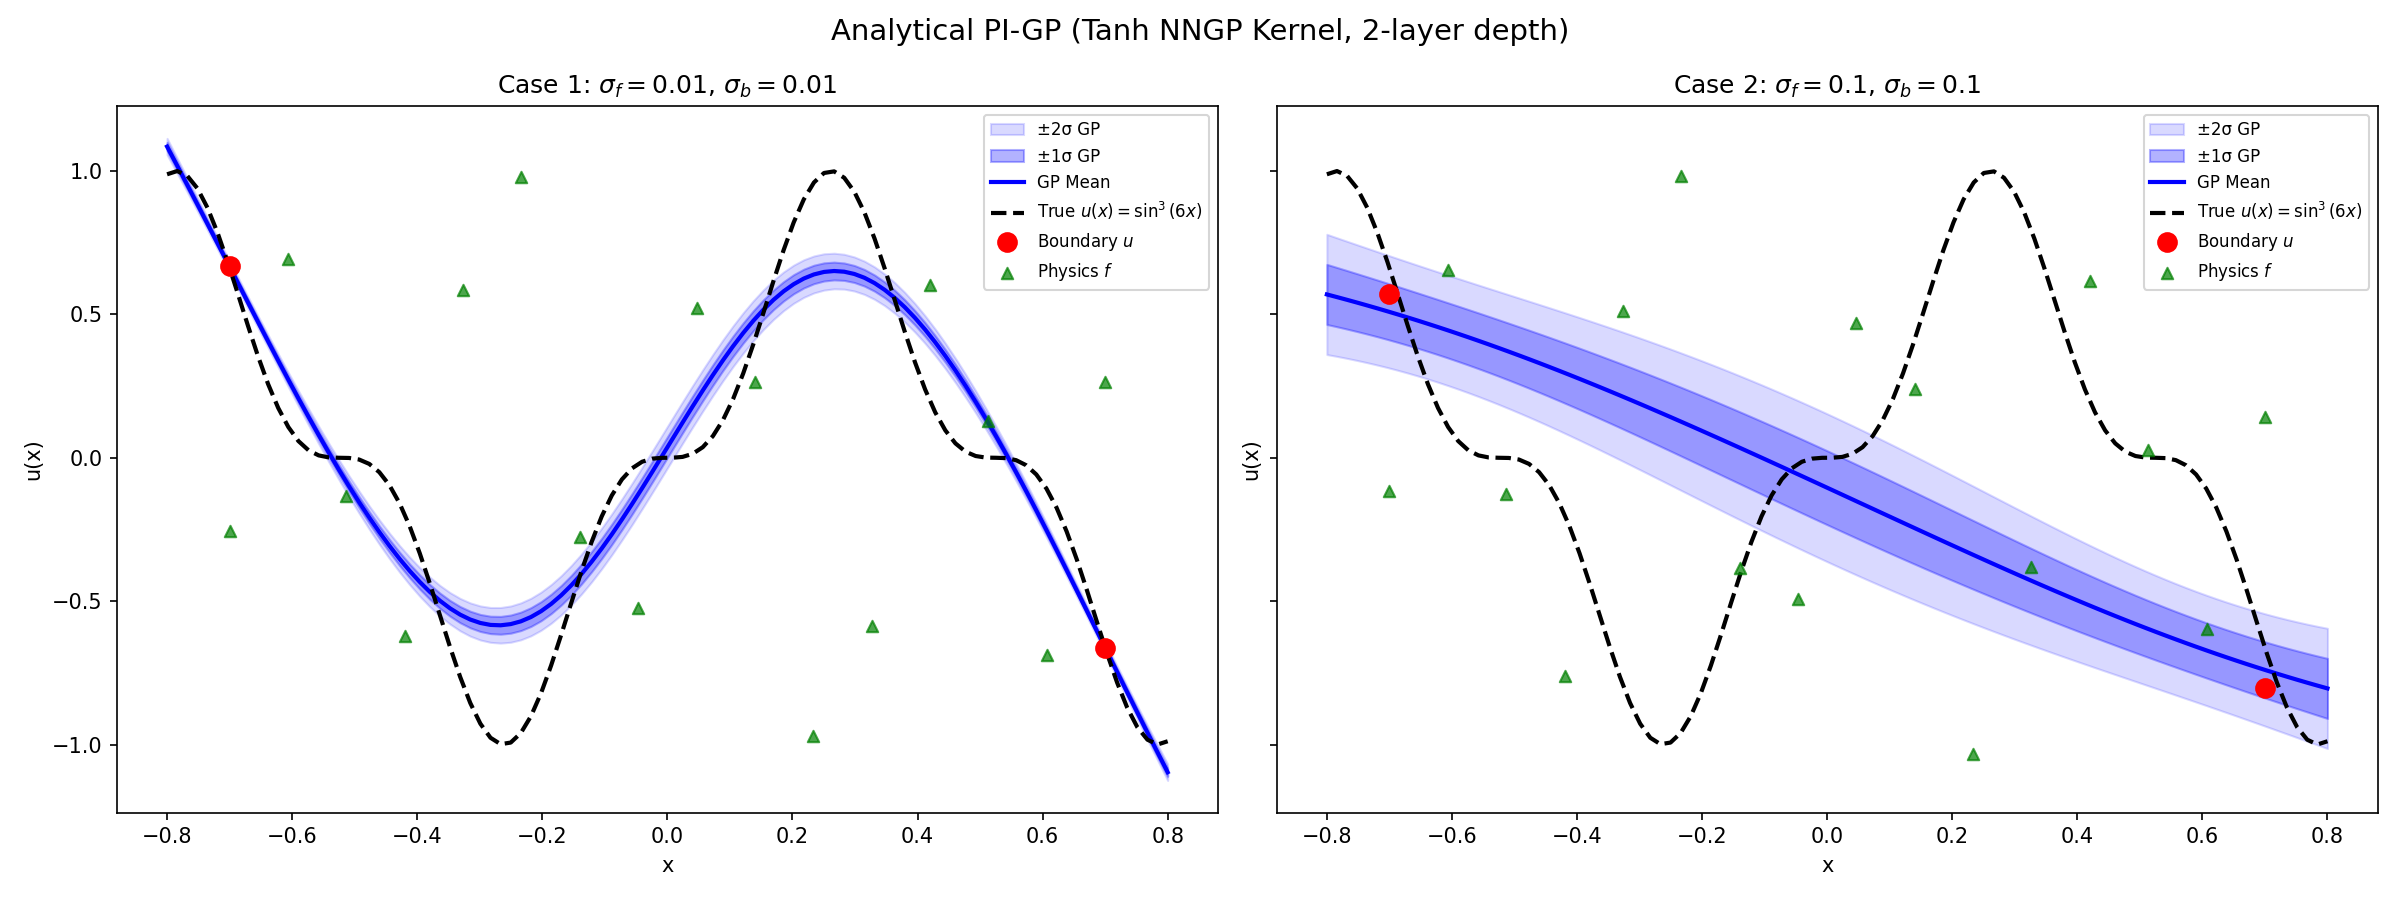
\includegraphics[width=\linewidth]{Figures/GP/test_gp_result.png}
                \caption{PI-GP posterior mean against truth $u(x) = \sin^3(6x)$ for low and high noise.}
            \end{figure}
        \end{column}
        \begin{column}{0.55\textwidth}
            \textbf{Failure of the PI-GP vs. Finite B-PINNs:}
            \begin{itemize}
                \item \textbf{Too Rigid:} The infinite-width limit forces the network to a "lazy regime" of NTK.
                \item \textbf{Smoothing effect:} This rigid structure causes the PI-GP to heavily over-smooth the physics in the presence of noise, missing the fast oscillating details of the wave.
                \item \textbf{Finite Networks Adapt:} Finite-width B-PINNs do not have fixed kernels. Their basis functions actively shift and adapt during training to perfectly align with sharp gradients and complex PDE dynamics.
            \end{itemize}
        \end{column}
    \end{columns}
\end{frame}

\section*{Conclusion}

% Slide 14
\begin{frame}{Conclusion}
    \begin{itemize}
        \item \textbf{B-PINNs $>$ PINNs for Noise:} HMC-driven B-PINNs successfully regularize against overfitting in chaotic PDE problems.
        \item \textbf{Metrics Matter:} Rigorous quantitative evaluation (PICP, MPIW) is crucial—visuals and Dropout are deceptive.
        \item \textbf{Dynamic Noise is Powerful:} Joint inference of noise (HBPINN) prevents numerical divergence and improves HMC sampling stability.
        \item \textbf{Finite vs Infinite (PI-GP):} While mathematically elegant, infinite-width exact PI-GPs fail on complex dynamics because their rigid kernels over-smooth. Finite-width B-PINNs are essential because their active representation learning can perfectly adapt to sharp features.
    \end{itemize}
\end{frame}


% Slide 16 (References)
\begin{frame}[allowframebreaks]{References}
    \bibliographystyle{plain}
    \bibliography{references}
\end{frame}

\end{document}
